%%%%%%%%%%%%%%%%%%%%%%%%%%%%%%%%%%%%%%%%%%%%%%%%%%%%%%%%%%%%%%%%%%%%%%
% How to use writeLaTeX: 
%
% You edit the source code here on the left, and the preview on the
% right shows you the result within a few seconds.
%
% Bookmark this page and share the URL with your co-authors. They can
% edit at the same time!
%
% You can upload figures, bibliographies, custom classes and
% styles using the files menu.
%
%%%%%%%%%%%%%%%%%%%%%%%%%%%%%%%%%%%%%%%%%%%%%%%%%%%%%%%%%%%%%%%%%%%%%%

\documentclass[12pt]{article}

\usepackage{sbc-template}

\usepackage{graphicx,url}

%\usepackage[brazil]{babel}   
\usepackage[utf8]{inputenc}  
%\usepackage[citestyle=authoryear,natbib=true,backend=bibtex]{biblatex}
%\usepackage[alf]{abntex2cite}
\usepackage[pdftex]{hyperref}
\usepackage[svgnames]{xcolor}
\usepackage{listings}

% \lstset{language=R,
%     basicstyle=\small\ttfamily,
%     stringstyle=\color{DarkGreen},
%     otherkeywords={0,1,2,3,4,5,6,7,8,9},
%     morekeywords={TRUE,FALSE},
%     deletekeywords={data,frame,length,as,character,recipe, step\_zv, step\_nzv, step\_normalize, step\_scale, decision_tree, workflow, fit, predict, mutate, metrics, print },
%     keywordstyle=\color{blue},
%     commentstyle=\color{DarkGreen},
%     numbers=yes,
%     numberstyle=\tiny\color{gray},
%     breaklines=true,
%     frame=tb
% }


     
\sloppy

\title{Aplicação do algoritmo de Árvore de Decisão para classificação de dados do uso de energia elétrica nos estados brasileiros}

\author{Danyelle da Silva Oliveira Angelo\inst{1}}


\address{Faculdade de Computação -- Universidade Federal de Uberlândia
  (UFU)\\
  \email{danyelle.angelo@ufu.br}
}

\begin{document} 

\maketitle
     
\begin{resumo}
    Neste trabalho aplicamos técnicas de machine learning (classificação), em um conjunto de dados que detalha a cadeia de energia elétrica do Brasil, com ênfase no consumo de energia elétrica por estado. O algoritmo escolhido para realizar a classificação desses dados foi o de árvore de decisão, apesar do alto grau de assertividade desse algoritmo, nossos resultados em termos de acurácia, não ultrapassaram o valor de 22\%, mostrando que o modelo construído não é a melhor para escolha para o problema delineado.
    
    
    %ser uma técnica de simples compreensão e implementação, ao mesmo tempo em que normalmente oferece alto grau de assertividade.
\end{resumo}


\section{Introdução}
    Dados abertos é um termo amplamente usado na sociedade, e está relacionado a disponização de dados e informações de caráter governamental e público na internet. Mas não basta tornar os dados disponíveis, é preciso que estes sejam processáveis e sigam um padrão. 
    
    De acordo com o portal \href{kit.dados.gov.br}{kit.dados.gov.br} \cite{kit-dados-abertos}, disponibilizar os dados governamentais de maneira padronizada permite:
    
    \begin{itemize}
        \item Economia de recursos: financeiro e de tempo, uma vez que o cidadão pode acessar as informações diretamente pela web, não há necessidade de protocolar uma ação junto à uma entidade.
        \item Redução de trabalho duplicado: os dados estando disponíveis, evita que outras equipes/entidades ou organizações, façam novamente a coleta de dados já existentes. Nessas situações os interessados podem reusar toda a base, ou até mesmo cruzar os dados já existentes, com novos dados;
        \item Conjuntos de dados podem ser combinados à conjuntos de dados de outras organizações, ampliando as possibilidades de trabalho sobre estes;
        \item Geração de empregos: a economia tende a ser estimulada, a medida que agentes econômicos  utilizem dados abertos para a criação de novos processos de negócio e na otimização dos já existentes.
    \end{itemize}

    Pode-se dizer assim, que a disponibilização e padronização desses dados, permitem a potencialização do valor dos conjuntos em si. Permitindo que diferentes setores da sociedade participem do desenvolvimento de políticas, análises, pesquisas, aplicações privadas ou públicas e processos de negócio.

    O site \href{dados.gov.br/}{https://dados.gov.br/} disponibiliza mais de 10.000 conjuntos de dados para pesquisa, de 218 instituições, esses dados são apresentados em diferentes formatos. É possível filtrar os conjuntos de dados disponíveis por organização, temas, etiquetas, licenças, ou formatos. Para a realização deste trabalho escolhemos trabalhar com um conjunto de dados que detalha o consumo de energia elétrica no país, nosso objetivo é classificar a unidade federativa (UF) de uma amostra com base nos valores de consumo, tipo de consumo, e região.
    
\section{Conjunto de dados} 

O conjunto de dados escolhido foi produzido no ano de 2018 e foi construído pela \textit{Empresa de Pesquisa Energética} (EPE). Conhecemos essa instituição através do  portal dados.gov.br, entretanto, apesar de haver uma página dedicada a EPE no portal citado, a mesma se encontra vazia (\href{https://dados.gov.br/organization/empresa-de-pesquisa-energetica-epe}{https://dados.gov.br/organization/empresa-de-pesquisa-energetica-epe}). Para ter acesso aos dados relativo ao consumo de energia elétrica no país é preciso acessar diretamente o site da EPE (\href{https://www.epe.gov.br/pt/publicacoes-dados-abertos/dados-abertos/dados-do-anuario-estatistico-de-energia-eletrica}{https://www.epe.gov.br/pt/publicacoes-dados-abertos/dados-abertos/dados-do-anuario-estatistico-de-energia-eletrica}). 
O conjunto disponibilizado no site da organização dá origem ao \textit{Anuário Estatístico de Energia Elétrica}, que tem por objetivo publicar informações do mercado de eletricidade no Brasil, sendo um excelente exemplo dos benefícios da disponibilização dos dados abertos, como dito anteriormente.

\subsection{Preparação dos dados}
Nosso conjunto de dados, possuí 483.759 observações, realizamos uma série de operações sobre o mesmo antes de aplicar o modelo de classificação escolhido. Para realizar estas operações fizemos o uso do pacote \textit{tidyverse}.

O \textit{tidyverse} agrupa uma série de ferramentas pertinentes ao processo de aprendizagem de máquina. Entre os pacotes suportados pelo tidyverse, usados neste trabalho temos: \textit{readr, dplyr} e  \textit{ggplot2}, sendo os 2 primeiros usados para leitura e manipulação de dados (respectivamente) e o segundo para a geração de gráficos (mostramos o uso desses pacotes na figura abaixo).
\begin{figure}[!h]
\centering
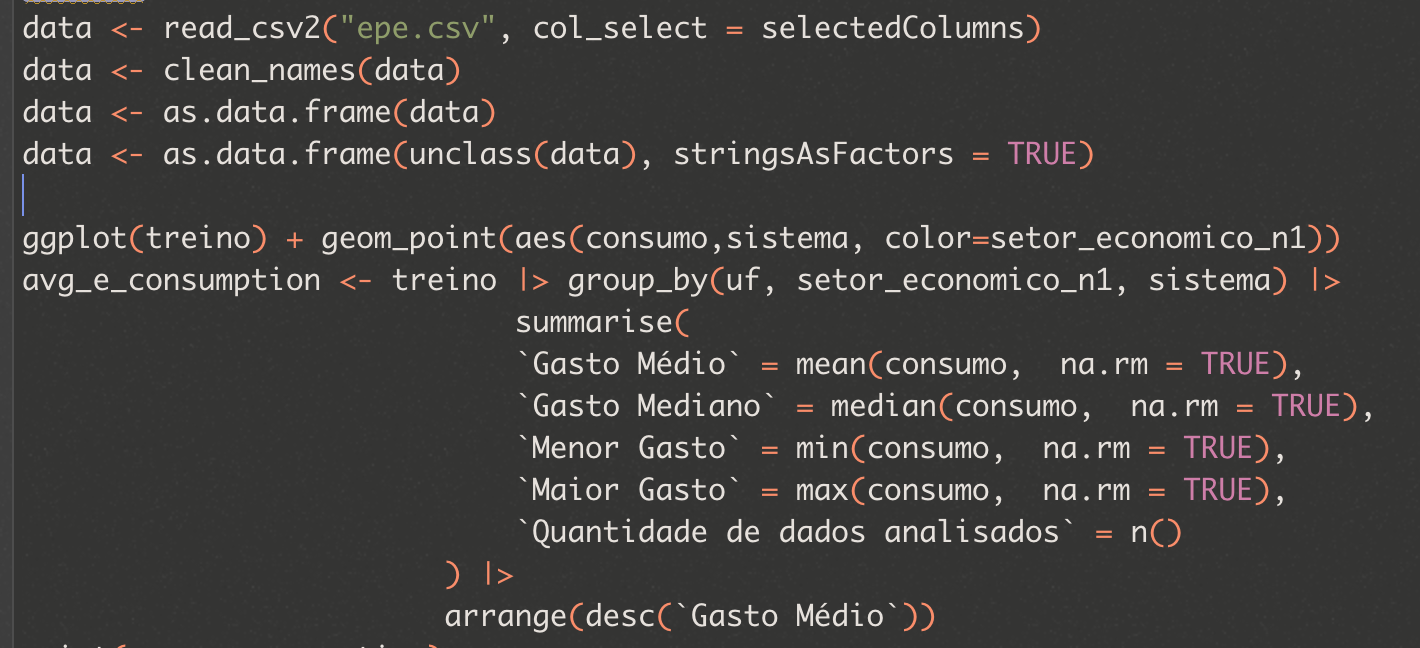
\includegraphics[width=1\textwidth]{images/tidyverse.png}
\caption{Carregando dados, gerando gráfico e resumindo dados com  tidyverse}
\label{fig:exampleFig1}
\end{figure}

Iniciamos o carregamento dos nossos dados (previamente baixados) através da função \textit{read\_csv2}, além do nome do arquivo que contém os dados, passamos também uma lista com as colunas que desejávamos carregar em nosso ambiente, excluindo assim atributos que não tinham variabilidade ou não apresentavam relevância para o nosso problema. 


Após formatar o conjunto de dados a ser analisado, utilizamos o pacote \textit{ggplot2} e posteriormente a função \textit{summarise} para entender a influência de cada atributo na base de dados.
Construímos um gráfico de pontos, que relaciona o consumo  de energia elétrica à uma região do país, categorizamos cada um desses pontos no gráfico através de cores, onde cada cor representa um setor econômico. Com a visualização do gráfico concluímos que as regiões com maior consumo de energia são a Sudeste e a Centro-Oeste, sendo que o tipo de consumo predominante é o Industrial.

\begin{figure}[!h]
\centering
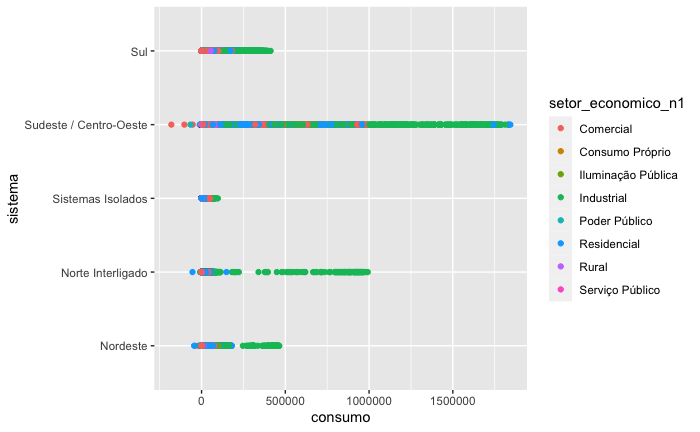
\includegraphics[width=1.2\textwidth]{images/consumo_sistema_tipoConsumo.png}
\caption{Tipo e valor de consumo energético por região}
\label{fig:exampleFig1}
\end{figure}


As conclusões acima, foram validadas através da sumarização dos dados da base de treino. Para realizar esse resumo dos dados agrupamos as amostras por estado (uf), tipo de consumo (setor\_economico\_n1) e região (sistema), após o agrupamento destes dados calculamos a mediana e média dos gatos, computamos também o maior e menor valor de gasto energético do agrupamento. Por fim, ordenamos estes dados em ordem decrescente de gasto médio. Os 10 agrupamentos com maior gasto energético (considerando tipo de gasto, e estado) são mostradas na Figura 3, e assim como inferimos do gráfico mostrado anteriormente, as regiões com maior consumo são Sudeste e Centro-Oeste.
\begin{figure}[!h]
\centering
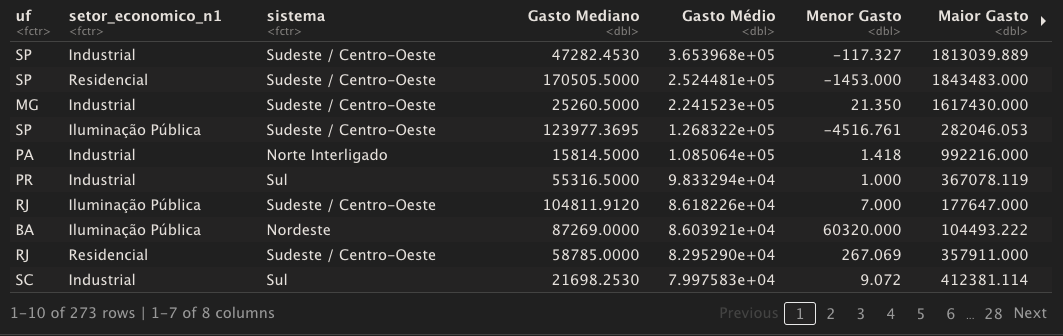
\includegraphics[width=1\textwidth]{images/summarise_treino.png}
\caption{Resumo dos dados}
\label{fig:exampleFig1}
\end{figure}

\section{Aprendizagem de máquina}
O problema proposto neste trabalho consiste em determinar o estado federativo (UF) relativo à uma amostra, dado uma região (sistema), Setor Econômico - N1, Setor Econômico - N2 e Taxa de Consumo elétrico. Sendo que os atributos Setor Econômico - N1 e Setor Econômico - N2 descrevem a classificação dos consumidores de energia elétrica de modo geral (o segundo é uma especificação do primeiro), são exemplos de classificação de consumo para os atributos citados acima:
\begin{itemize}
    \item N1: Comercial, Consumo Próprio, Industrial, Poder Público, Rural e Serviço Público e etc;
    \item N2: Adm. Condominial, Iluminação, Uso Comum, Serviços de Comunicações e Telecomunicações, Templos Religiosos, Agroindústria, Escola Agrotécnica e etc.
\end{itemize}

Para realizar a classificação das nossas amostras, utilizamos o algoritmo de Árvore de decisão. Nesse algoritmo cada nó interno representa um teste de valor de um dos atributos das observações, e os nós folhas representam o resultado final da decisão, ou seja a classificação da amostra.

Com o uso do pacote \textit{tidymodels} modelamos nossos dados, para aplicar o algoritmo de aprendizagem de máquina.
\begin{enumerate}
    \item Separamos nossos dados de treino e de teste (80\% para treino e 20\% para teste);
    \item Criamos uma especificação (receita) para o nosso modelo;
    \item Definimos um modelo, no caso a escolha foi a árvore de decisão;
    \item Criamos um fluxo de trabalho: esse processo é a junção do modelo definido com a receita;
    \item E por fim executamos e medimos a qualidade do nosso classificador.
\end{enumerate}
A imagem abaixo, traz o trecho do código em R, responsável pelos passos citados:

\begin{figure}[!h]
\centering
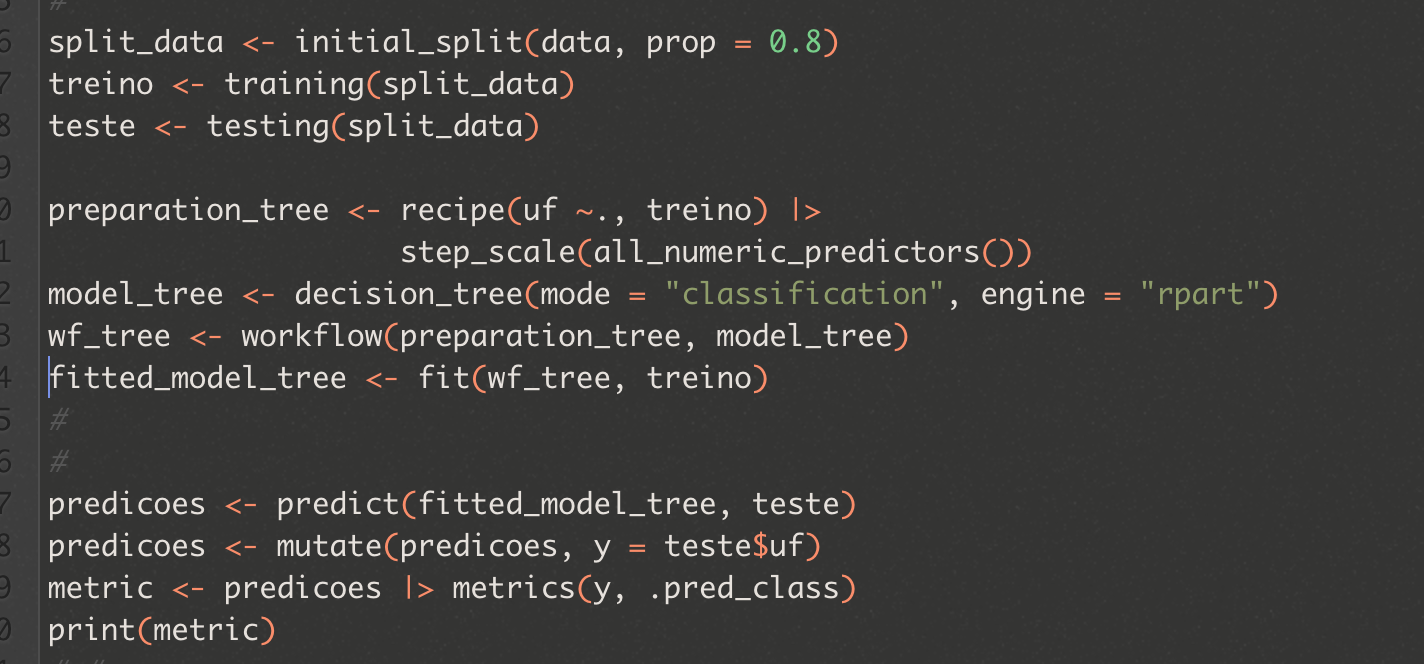
\includegraphics[width=1\textwidth]{images/tidymodels.png}
\caption{Preparação dos dados, criação e aplicação do modelo}
\label{fig:exampleFig1}
\end{figure}

\newpage

\section{Experimentos e Resultados}
Como relatado, a base de dados escolhida tem 483.759 informações, as configurações da máquina utilizada para os experimentos são:
\begin{itemize}
    \item Processador: Intel core i7 de 2,6 GHz
    \item Memória: 16GB de 2667 MHz
    \item Sistema Operacional: macOS Monterey
\end{itemize}
Como a tarefa considerada mais díficil é criar as regras de decisão da nossa árvore, dedicamos uma porção maior do nosso conjunto de dados para o processo de treino. Assim 20\%  foi usado no processo de validação (teste) do modelo contruído, e 80\% foi destinado para o treino. Nossa acurácia se manteve perto de 21\%, não chegando à um resultado satisfatório.

\section{Considerações Finais}
Neste trabalho, escolhemos um conjunto de dados governamental com característica de consumo de energia elétrica por região, nosso objetivo era classificar o estado a qual uma amostra pertence, de acordo com os seguintes atributos: região, tipo de consumo, especificação do tipo de consumo, e nível de consumo energético. 

Para fazer essa classificação utilizamos o algoritmo de aprendizagem de máquina de Árvore de Decisão.  Não alcançamos o resultado esperado, devido a baixa acurácia do nosso modelo. Como trabalho futuro queremos averiguar a influência do algoritmo de k-vizinhos mais próximos na acurácia do problema proposto.


\bibliographystyle{sbc}
\bibliography{sbc-template}
\end{document}


